\documentclass{article}
\usepackage[utf8]{inputenc}
\usepackage[spanish]{babel}
\usepackage{listings}
\usepackage{graphicx}
\graphicspath{ {images/} }
\usepackage{cite}
\usepackage{hyperref}
\usepackage{amssymb, amsmath}
\usepackage{geometry}
\geometry{
textheight=23cm
}

%arduino
\input{arduinoLanguage.tex}    % adds the arduino language listing

%% Define an Arduino style fore use later %%
\lstdefinestyle{myArduino}{
  language=Arduino,
  %% Add other words needing highlighting below %%
  morekeywords=[1]{},                  % [1] -> dark green
  morekeywords=[2]{FILE_WRITE},        % [2] -> light blue
  morekeywords=[3]{SD, File},          % [3] -> bold orange
  morekeywords=[4]{open, exists},      % [4] -> orange
  %% The lines below add a nifty box around the code %%
  frame=shadowbox,
  rulesepcolor=\color{arduinoBlue},
}

\begin{document}

\begin{titlepage}
    \begin{center}
        \vspace*{1cm}
            
        \Huge
        \textbf{Parcial 1: Informática II}
            
        \vspace{0.5cm}
        \LARGE
       Análisis y diseño.
          
            
        \vspace{6cm}
        
        \textbf{JOSE MIGUEL GOMEZ MONSALVE}
        
        \vspace{0.5cm}
        
        \textbf{ERIKA DAYANA LEÓN QUIROGA}
        
        \vspace{0.5cm}
        
        \textbf{DAVID AGUDELO OCHOA}
            

            
        \vfill
            
        \vspace{0.8cm}
       
        \Large


        \vfill
        Despartamento de Ingeniería Electrónica y Telecomunicaciones\\
        Universidad de Antioquia\\
        Medellín\\
        Febrero 2022
                 
    \end{center}
\end{titlepage}


\tableofcontents\newpage

\section{Introducción.}\label{intro}
En el siguiente informe se verán los pasos realizados para la solución de un problema en específico, este problema es la desencriptación de un mensaje. El mensaje encriptado llegará en forma de arreglo y, mediante una clave, el programa identificará el mensaje real. Para la solución del problema se investigó el uso del integrado 74HC595, el cual nos permitirá paralelizar los datos que llegarán desde el arduino emisor, y de esta forma minimizar el uso de puertos seriales en el arduino receptor, además de permitirnos comprobar la llegada de la clave por medio del llamado "Bloque de desencriptacion", el cual está implementado con compuertas lógicas. El arduino receptor será el encargado de mostrar por medio de una pantalla LCD el mensaje desencriptado.

\section{Integrado 74HC595.} \label{Integrado}
El integrago 74HC595 hace parte de la familia de dispositivos SNx4HC59, la cual contienen un registro de desplazamiento de 8 bits de entrada en serie y salida en paralelo, el registro de almacenamiento tiene salidas de 3 estados paralelos. Se proporcionan relojes separados para el registro de desplazamiento y el de almacenamiento. El registro de desplazamiento tiene una entrada de anulación directa (SRCLR), una entrada en serie (SER) y salidas en serie para la conexión en cascada. Tienen una amplia corriente de funcionamiento de 2 V a 6 V, y las salidas de 3 estados de alta corriente pueden controlar hasta 15 cargas LSTTL. Los dispositivos tienen un bajo consumo consumo de 80-uA (máximo) ICC.
\subsection{Características del integrado.}\label{caracteristicas}
 \begin{itemize}
 
\item Entrada serial, salida paralela, o salida serial que permite la conexión en cascada de varios integrados.
\item Registro de desplazamiento de 8 bits que alimenta a un registro de almacenamiento.
\item Entradas de reloj separadas para el registro de desplazamiento y el de almacenamiento con activación por flanco de subida.

\end{itemize}

\begin{figure}[h]
\includegraphics[scale=1]{esquematico.png}
\centering
\caption{Integrado 74HC595.}
\label{fig:int74HC959}
\end{figure}

\begin{figure}[h]
\includegraphics[scale=0.5]{circuitoconexion.png}
\centering
\caption{Circuito de conexión esquemático 74HC595.}
\label{fig:Circuito de conexión esquemético}
\end{figure}

\begin{table}
\centering
\begin{tabular}{lll}
\textbf{Número pin} & \textbf{Nombre del pin}       & \textbf{Descripción}                                              \\
1,2,3,4,5,6,7       & Pines de salida (de Q1 a Q7)  & Salidas del integrado  \\
8                   & GND                        & Tierra                                                \\
9                   & (P7) Salida en serie          & Conexion de más de un 74hc595 en cascada                          \\
10                  & (MR) Restablecimiento maestro & Restablece todas las salidas como bajas.                          \\
11                  & (SH\_CP) Reloj                & Reloj que sincroniza la carga de datos.                                          \\
12                  & (ST\_CP) Pestillo             & Se utiliza para actualizar los datos a los pines de salida.        \\
13                  & (OE) Activación de salida     & Se utiliza para desactivar las salidas.                           \\
14                  & (DS) Datos en serie           & Este es el pin al que se envían los datos                          \\
15                  & (P0) salida                   & El primer pasador de salida.                                      \\
16                  & Vcc                           & Este pin alimenta el IC                                          
\end{tabular}
\end{table}

\subsection{Funcionamiento.}\label{integrado funcionamiento}
El objetivo principal es pasar el número dado de un formato serial a uno parelelo. Para explicar el funcionamiento del integrado tomaremos un número cualquiera de 8 bits, este número se irá guardando bit por bit en cada uno de los cuadros que se pueden ver en la Figura \ref{fig:func1}, también podemos ver en esta misma figura que la entrada de los datos es en serie (uno por uno), y la salida de ellos es en paralelo (8 bits).

\newpage

\begin{figure}[h]
\includegraphics[scale=0.8]{funcionamiento1.png}
\centering
\caption{Representación del funcionamiento del circuito integrado 74HC595.}
\label{fig:func1}
\end{figure}

Para que la toma de los datos sea exitosa es necesario un reloj que por medio de pulsos, controlará en qué momento ingresa al integrado el bit presente en la entrada. Tomaremos de ejemplo la representación binaria del número 49, la cual es 00110001.

El primer paso para transformar la información que se encuentra en serie a paralelo es realizar el desplazamiento de los bits dentro del integrado iniciando por el bit más significativo (MSB por sus siglas en inglés), en nuestro ejemplo es un cero, que se encuentra presente en la entrada y que en el primer pulso del rejol ingresa a la primera posición del registro de desplazamiento. Figura \ref{fig:MSB}

\begin{figure}[h]
\includegraphics[scale=0.8]{MSB.png}
\centering
\caption{Entrada del MSB al integrado.}
\label{fig:MSB}
\end{figure}

En el próximo pulso del reloj el MSB, ya dentro del integrado, se correrá una posición a la derecha en el registro de desplazamiento, mientras que el número a la derecha del MSB, en la entrada, se posicionará en la primera posición del registro de desplazamiento.


\begin{figure}[h]
\includegraphics[scale=0.8]{MSB1.png}
\centering
\caption{Desplazamiento de los bits dentro del integrado.}
\label{fig:MSB1}
\end{figure}

Este proceso se repetirá hasta que se ingrese al registro de desplazamiento el último bit del número (Figura \ref{fig:registrolleno}).

\begin{figure}[h]
\includegraphics[scale=0.8]{BitsDespla.png}
\centering
\caption{Desplazamiento de los bits dentro del integrado.}
\label{fig:bitsdespla}
\end{figure}

\newpage
\begin{figure}[h]
\includegraphics[scale=0.8]{registrolleno.png}
\centering
\caption{Registro de desplazamiento lleno. Se utilizaron colores encima o abajo de los bits para identificar fácilmente cuál es cuál en el registro de desplazamiento.}
\label{fig:registrolleno}
\end{figure}

Para que las salidas no vayan cambiando mientras que el registro de desplazamiento se llena, el integrado hace uso del registro de almacenamiento y el RCLK (Rejol del registro de almacenamiento). Figura \ref{fig:registroalmacenamiento}

\begin{figure}[h]
\includegraphics[scale=0.6]{regisalmacen.png}
\centering
\caption{Representación del registro de almacenamiento.}
\label{fig:registroalmacenamiento}
\end{figure}

Una vez se finalice la carga de datos en el registro de desplazamiento, con un único pulso del RCLK se cargan todos los datos del registro de desplazamiento al registro de almacenamiento y se muestran en la salida. De esta forma se alcanzará el objetivo principal, transformar los datos de entrada en serie a datos de salida paralelos.

\newpage
\begin{figure}[h]
\includegraphics[scale=0.8]{salida.png}
\centering
\caption{Representación del registro de almacenamiento.}
\label{fig:salida}
\end{figure}


\subsection{Aplicaciones.}\label{Aplicaciones}
\begin{itemize}
\item Network switches
\item Power infrastructure
\item LED displays
\item Servers
\end{itemize}

\newpage
\subsection{Uso del Circuito Integrado 74HC595.}\label{Usocircuito}

\begin{itemize}
\item Con pulsadores: 

\begin{figure}[h]
\includegraphics[scale=0.6]{pulsadores.png}
\centering
\caption{Circuito con integrado 74HC595 haciendo uso de pulsadores.}
\label{fig:pulsadores}
\end{figure}

El montaje del circuito utilizando el 74HC595 realizado con pulsadores utiliza los conceptos vistos en la sección en donde se explica el funcionamiento del integrado. 
Se utiliza un interruptor deslizante para la entrada serial (SER), y dos pulsadores o switches que harán el trabajo de los relojes (SRCLK y RCLK). Si el interruptor deslizante está posicionado a la izquierda significa que entra un cero, si está posicionado a la derecha, es un uno. 
Para realizar la entrada de los datos al integrado, se desliza el interruptor SER hacia el lado del dato que necesito ingresar, después de esto se hace la activación del reloj del registro de desplazamiento (SRCLK) oprimiendo el switch con este nombre una vez, de esta forma se subirá el primer dato. Para el segundo dato se realizá el mismo procedimiento: se desliza el interruptor con el nombre SER hacia el lado del dato que requiere ingresar (izquierda cero, derecha uno) y posterior a esto se oprime una vez el interruptor llamado SRCLK. Este proceso se realiza hasta que ingrese los ocho datos que puede almacenar el integrado 74HC595, cuando termine de ingresar los datos se procede a oprimir el interruptor llamado RCLK, el cuál mandará los datos almacenados en el integrado hacia las salidas, por lo que el número ingresado se verá reflejado en los LEDs incluidos en el circuito.

La simulación se puede probar utilizando el siguiente link: \url{https://www.tinkercad.com/things/iBjAIisXge3}

\newpage
\item Con arduino: 

\begin{figure}[h]
\includegraphics[scale=0.4]{prueba arduino integrado.png}
\centering
\caption{Circuito con integrado 74HC595 haciendo uso de un arduino.}
\label{fig:reemplazo pulsador por arduino}
\end{figure}

\begin{lstlisting}[style=myArduino]
//directivas de preprocesamiento
#define tiempo 2000
#define SER 2
#define RCLK 3
#define SRCLK 4


byte codigo[8]={10,255,0,49,50,6,7,8};//A byte stores an 8-bit unsigned number, from 0 to 255.
//----------------------------------------------------------------
//prototipo de las funciones

//----------------------------------------------------------------
//setup
void setup()
{
  for(int i=2;i<5;i++)
  {
    pinMode(i, OUTPUT);
  }
  
}
//----------------------------------------------------------------
//loop
void loop()
{
  for(int i=0;i<8;i++)
  {
  	//delay(25);
    for(int j=0;j<8;j++)
    {
      digitalWrite(SRCLK, LOW);
      digitalWrite(SER, bitRead(codigo[i], j));
      digitalWrite(SRCLK, HIGH);
    }
    //delay(tiempo-25);
    delay(tiempo);
    digitalWrite(RCLK, HIGH);
    digitalWrite(RCLK, LOW);
    
  }
  
  
  
}
//----------------------------------------------------------------
//cuerpo de las funciones
\end{lstlisting}

Como podemos ver, el montaje con arduino se realiza mediante tres pines digitales, que van conectados al SER, SRCLK y RCLK, el control de estos pines se realiza mediante código escrito con lenguaje C++.
Definimos los nombres de los pines para que sea más sencillo utilizarlos a la hora de realizar el programa que nos controlará el circuito integrado. Con un for haremos el SETUP de todos los pines digitales como salidas. En el loop se mandará la información al SER, controlado por el pin digital 2, utilizando la función bitRead, la cual nos dará un número cualquiera en binario y así lo podremos ingresar al circuito integrado. El pin digital 4 controlará el reloj de registro de desplazamiento, el cual irá guardando bit a bit el número binario en el circuito integrado, y el pin digital 3 controlará el reloj de registro de salida, que una vez activado mandará los datos guardados en el circuito integrado a las salidas.

\end{itemize}


\vspace{0.5cm}
\noindent


\section{Comunicación entre Arduinos} \label{Comunicación entre Arduinos}
\subsection{Prueba 1}\label{intento1}
A continuación se presenta el código y montaje de arduinos que se usaron para probar el tema de comunicación entre dos arduinos. Cabe aclarar que la implementación de estos se dio antes de las indicaciones y especificaciones de la clase del día 17 de febrero, por lo que no reflejan el futuro diseño a implementar, el cual contará con una gran participación del integrado 74HC595 y se sospecha que también del protocolo I2C para la señal de reloj.

\subsubsection{Arduino emisor.}\label{intento1}

código:
\begin{lstlisting}[style=myArduino]//directivas de preprocesamiento
#define tiempo 1000
byte codigo[8]={1,2,3,4,5,6,7,8};//A byte stores an 8-bit unsigned number, from 0 to 255.
//----------------------------------------------------------------
//prototipo de las funciones

//----------------------------------------------------------------
//setup
void setup()
{
  for(int i=2;i<11;i++)
  {
    pinMode(i, OUTPUT);
  }
  
}
//----------------------------------------------------------------
//loop
void loop()
{
  for(int i=0;i<8;i++)
  {
  	digitalWrite(10, LOW);
  	delay(25); // Wait for 1000 millisecond(s)
    for(int j=0;j<8;j++)
    {
      digitalWrite(j+2, bitRead(codigo[i], j));
    }
    delay(tiempo-25);
    digitalWrite(10, HIGH);
    delay(tiempo);
  }
  
  
}
//----------------------------------------------------------------
//cuerpo de las funciones
\end{lstlisting}

montaje:
\begin{figure}[h]
\includegraphics[scale=0.6]{emisor1.png}
\centering
\caption{Prueba de emisión de bits y una señal de reloj por medio de 9 leds.}
\label{fig:emisor1}
\end{figure}

\newpage
\subsubsection{Conexión entre arduino emisor y receptor}\label{intento1}

montaje:
\begin{figure}[h]
\includegraphics[scale=0.6]{emisorReceptor1.png}
\centering
\caption{Prueba de emisión de bits y una señal de reloj por medio de 9 leds y su recepción a otro arduino.}
\label{fig:emisorReceptor1}
\end{figure}

código arduino emisor:
\begin{lstlisting}[style=myArduino]//directivas de preprocesamiento
//directivas de preprocesamiento
#define tiempo 250
byte codigo[8]={2,1,3,4,5,6,7,8};//A byte stores an 8-bit unsigned number, from 0 to 255.
//----------------------------------------------------------------
//prototipo de las funciones

//----------------------------------------------------------------
//setup
void setup()
{
  for(int i=2;i<11;i++)
  {
    pinMode(i, OUTPUT);
  }
  
}
//----------------------------------------------------------------
//loop
void loop()
{
  for(int i=0;i<9;i++)
  {
  	digitalWrite(10, LOW);
  	delay(50); // Wait for 1000 millisecond(s)
    for(int j=0;j<8;j++)
    {
      digitalWrite(j+2, bitRead(codigo[i], j));
    }
    delay(tiempo-50);
    digitalWrite(10, HIGH);
    delay(tiempo);
  }
  
  
}
//----------------------------------------------------------------
//cuerpo de las funciones
 
\end{lstlisting}

código arduino receptor:
\begin{lstlisting}[style=myArduino]//directivas de preprocesamiento
// C++ code
//
int entero=0;
bool primerCero=false;
void setup()
{
  Serial.begin(9600);
  for(int i=2;i<11;i++)
  {
    pinMode(i, INPUT);
  }
}

void loop()
{
  if(primerCero==true)
  {
    for(int i=0;i<8;i++)
    {
      entero=entero+((int)digitalRead(i+2))*pow(2,i);
    }
    Serial.println(entero);
    entero=0;
    primerCero=false;
  }
  if(primerCero==false)
  {
    while(digitalRead(10)==true)
    {
      primerCero=true;
    }
  }
  
}
 
\end{lstlisting}

\subsection{Prueba 2: Protocolo I2C}\label{intento2}
A continuación se presenta un modelo más cercano a lo que se planea hacer para la comunicación de la señal de reloj y los datos. Para ello usaremos el protocolo I2C.

montaje:
\begin{figure}[h]
\includegraphics[scale=0.5]{emisorReceptor2.png}
\centering
\caption{Comunicación mediante el protocolo I2C.}
\label{fig:emisorReceptor2}
\end{figure}

Código arduino emisor:
\begin{lstlisting}[style=myArduino]//directivas de preprocesamiento
#include <Wire.h>

// C++ code
//----------------------------------------------------------------
//----------------------------------------------------------------

byte pin[] = {9, 10, 11, 12, 13};
byte estado = 0;
#define retardo 2000
int ValorSensor = 0;

//----------------------------------------------------------------
//----------------------------------------------------------------

void setup()
{
  Wire.begin();
  pinMode(LED_BUILTIN, OUTPUT);
}

//----------------------------------------------------------------
//----------------------------------------------------------------

void loop()
{
  Wire.beginTransmission(1); // Transmite al Esclavo 1
  Wire.write(estado);
  Wire.endTransmission();
  
  digitalWrite(LED_BUILTIN, estado);
  
  delay(retardo);
  
  if (estado == 0)
  {
    estado = 1;
  }
  else
  {
    estado = 0;
  }
}
 
\end{lstlisting}

Código arduino receptor:
\begin{lstlisting}[style=myArduino]//directivas de preprocesamiento
#include <Wire.h>

void llegaDato(int howMany);
// C++ code
//
void setup()
{
  pinMode(13, OUTPUT);    // Pines en modo salida
  Wire.begin(1); // Unimos este dispositivo al bus I2C con dirección 2 (Esclavo 2)
  Wire.onReceive(llegaDato);
  pinMode(LED_BUILTIN, OUTPUT);
}

void loop()
{
  delay(30); // Wait for 1000 millisecond(s)
}

void llegaDato(int howMany){  
  int estado = 0;
  if (Wire.available() == 1) // Si hay un byte disponible
  {
    estado = Wire.read();
  }
  digitalWrite(13,estado);   // Activamos/desactivamos salida depende del Maestro
}
 
\end{lstlisting}

\subsection{Prueba 3: Conexión entre arduinos usando puertos digitales}\label{intento3}
Tras la sesión de clase del día 25 de febrero, el profesor nos indicó que no había necesidad de recurrir a protocolos como el I2C, por lo que se procedió a hacer una implementación mediante el uso de puertos digitales únicamente. \newline A continuación se presenta primeramente el montaje del uso del circuito integrado 74HC595, para probar así el proceso de emisión del arduino generador , y el proceso de recepción del segundo arduino, a la vez que verificamos con el integrado.
\newline Montaje: \newline \newline \newline

\begin{figure}[h]
\includegraphics[scale=0.6]{prueba conexión entre arduinos (fallo).png}
\centering
\caption{Comunicación entre arduinos, verificando con la ayuda de 8 leds y el integrado.}
\label{fig:reemplazo pulsador por arduino}
\end{figure}
Lastimosamente, no se pudo codificar de forma correcta, por lo que el proceso de recepción falló.
\newline Código emisor:
\begin{lstlisting}[style=myArduino]
//directivas de preprocesamiento
#define tiempo 2000
#define SER 2
#define RCLK 3
#define SRCLK 4


byte codigo[8]={10,255,0,49,50,6,7,8};//A byte stores an 8-bit unsigned number, from 0 to 255.
//----------------------------------------------------------------
//prototipo de las funciones

//----------------------------------------------------------------
//setup
void setup()
{
  for(int i=2;i<5;i++)
  {
    pinMode(i, OUTPUT);
  }
  
}
//----------------------------------------------------------------
//loop
void loop()
{
  for(int i=0;i<8;i++)
  {
  	//delay(25);
    for(int j=0;j<8;j++)
    {
      digitalWrite(SRCLK, LOW);
      digitalWrite(SER, bitRead(codigo[i], j));
      digitalWrite(SRCLK, HIGH);
    }
    //delay(tiempo-25);
    delay(tiempo);
    digitalWrite(RCLK, HIGH);
    digitalWrite(RCLK, LOW);
    
  }
  
  
  
}
//----------------------------------------------------------------
//cuerpo de las funciones
\end{lstlisting}

Código receptor:
\begin{lstlisting}[style=myArduino]
#define SER 2
#define RCLK 3
#define SRCLK 4

void setup()
{
  Serial.begin(9600);
  for(int i=2;i<5;i++)
  {
    pinMode(i, INPUT);
  }

}

void loop()
{
  if(digitalRead(RCLK))
  {
    if(digitalRead(SRCLK))
    {
      for(int i=0;i<8;i++)
      {
        Serial.print(digitalRead(2));
      }
      Serial.println();
    }
  }
}
\end{lstlisting}

\subsubsection{Conexión entre arduinos usando puertos digitales.}\label{intento4}
Tras varias horas de prueba se consigue una comunicación exitosa entre ambos arduinos, no solo mostrando los números en formato binario, sino también en décimal. (el montaje es el mismo del intento número 3).

Código emisor:
\begin{lstlisting}[style=myArduino]
//directivas de preprocesamiento
#define tiempo 1000
#define SER 2
#define RCLK 3
#define SRCLK 4


byte codigo[8]={1,2,255,0,50,6,7,8};//A byte stores an 8-bit unsigned number, from 0 to 255.
int tamanoArray=sizeof(codigo)/sizeof(byte);
//----------------------------------------------------------------
//prototipo de las funciones

//----------------------------------------------------------------
//setup
void setup()
{
  for(int i=2;i<5;i++)
  {
    pinMode(i, OUTPUT);
    digitalWrite(i, LOW);
  }
}
//----------------------------------------------------------------
//loop
void loop()
{
  for(int i=0;i<tamanoArray;i++)
  {
    for(int j=0;j<8;j++)
    {
      digitalWrite(SER, bitRead(codigo[i], j));
      digitalWrite(SRCLK, HIGH);
      delay(100);
      digitalWrite(SRCLK, LOW);

    }
    delay(tiempo);
    digitalWrite(RCLK, HIGH);
    digitalWrite(RCLK, LOW);
    
  }
  
  
  
}
//----------------------------------------------------------------
//cuerpo de las funciones
\end{lstlisting}

Código receptor:
\begin{lstlisting}[style=myArduino]
#define SER 2
#define RCLK 3
#define SRCLK 4

bool leerBit=true;
byte binario[8];

byte bintodec(byte* bin);
byte dos_exp (int exp);

void setup()
{
  Serial.begin(9600);
  for(int i=2;i<5;i++)
  {
    pinMode(i, INPUT);
  }
}

void loop()
{
  
  if(digitalRead(SRCLK))
  {
    for(int i=0;i<8;i++)
    {
      while(!digitalRead(SRCLK))
      {
        
      }
      binario[i]=digitalRead(SER);
      while(digitalRead(SRCLK))
      {
        
      }
    }
    delay(1000);
    for(int i=7;i>=0;i--)
    {
      Serial.print(binario[i]);
    }
    Serial.println();
    Serial.println(bintodec(binario));
  }
}
//--------------------------------------------------------------
//funciones
byte bintodec(byte * bin){ // recibe un binario y retorna un decimal en tipo entero
    byte dec = 0;
    for(int i=7; i>=0 ; i--){
        if (bin[i]>=1){
                dec = dec + (dos_exp(i));
        }
    }
    return dec;
}

byte dos_exp (int exp){
    int acu = 1;
    for (int i=0 ; i<exp ; i++){
        acu = acu*2;
    }
    return acu;
}
\end{lstlisting}

Salida por monitor serial:
\begin{figure}[h]
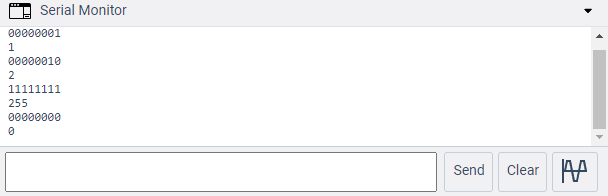
\includegraphics[scale=0.6]{salida monitor serial.png}
\centering
\caption{Salida monitor serial mostrando la recepción tanto en binario como en decimal.}
\label{fig:reemplazo pulsador por arduino}
\end{figure}
\subsubsection{Conexión entre arduinos: Pantalla LCD}\label{intento4}
Una vez funciona la comunicación entre arduinos, se procede a traspasar el codigo, de modo que el despliegue de información pase del monitor serial, como venía mostrándose, a un display lcd.

Montaje:

\begin{figure}[h]
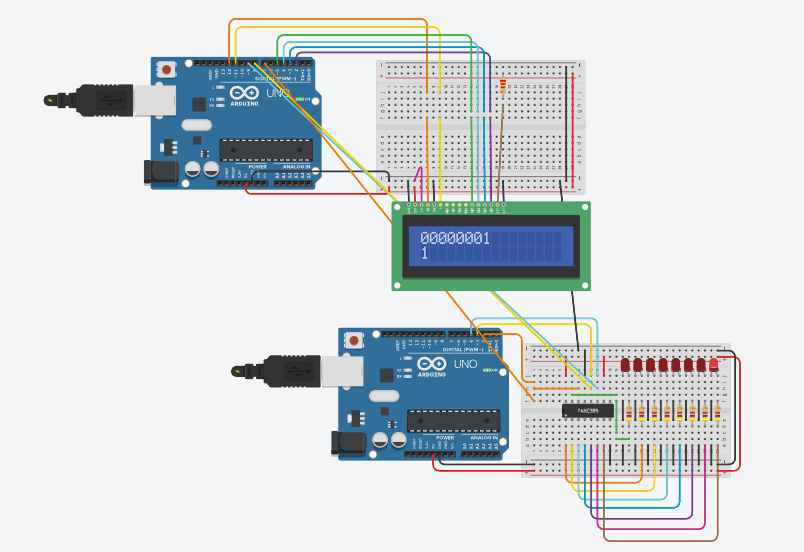
\includegraphics[scale=0.6]{implementacion lcd bin y dec.png}
\centering
\caption{Conexión arduinos con lcd.}
\label{fig:reemplazo pulsador por arduino}
\end{figure}

\newpage
Código emisor:
\begin{lstlisting}[style=myArduino]
//directivas de preprocesamiento
#define tiempo 1000
#define SER 2
#define RCLK 3
#define SRCLK 4


byte codigo[8]={1,2,255,0,50,6,7,8};//A byte stores an 8-bit unsigned number, from 0 to 255.
int tamanoArray=sizeof(codigo)/sizeof(byte);
//----------------------------------------------------------------
//prototipo de las funciones

//----------------------------------------------------------------
//setup
void setup()
{
  for(int i=2;i<5;i++)
  {
    pinMode(i, OUTPUT);
    digitalWrite(i, LOW);
  }
}
//----------------------------------------------------------------
//loop
void loop()
{
  for(int i=0;i<tamanoArray;i++)
  {
    for(int j=0;j<8;j++)
    {
      digitalWrite(SER, bitRead(codigo[i], j));
      digitalWrite(SRCLK, HIGH);
      delay(100);
      digitalWrite(SRCLK, LOW);

    }
    delay(tiempo);
    digitalWrite(RCLK, HIGH);
    digitalWrite(RCLK, LOW);
    
  }
  
  
  
}
//----------------------------------------------------------------
//cuerpo de las funciones
\end{lstlisting}

Código receptor:
\begin{lstlisting}[style=myArduino]
// include the library code:
#include <LiquidCrystal.h>

// initialize the library with the numbers of the interface pins
LiquidCrystal lcd(12, 11, 5, 4, 3, 2);

#define SER 7
#define RCLK 8
#define SRCLK 9

byte bintodec(byte * bin);
byte binario[8];

byte dos_exp (int exp);

void setup() {
  // set up the LCD's number of columns and rows:
  lcd.begin(16, 2);
  
  for(int i=7;i<10;i++)
  {
    pinMode(i, INPUT);
  }
}

void loop() {
  
  if(digitalRead(SRCLK))
  {
    for(int i=0;i<8;i++)
    {
      while(!digitalRead(SRCLK))
      {
        
      }
      //Serial.print(digitalRead(2));
      binario[i]=digitalRead(SER);
      while(digitalRead(SRCLK))
      {
        
      }
    }
    delay(1000);
    lcd.clear();
    for(int i=7;i>=0;i--)
    {
      lcd.print(binario[i]);
    }
    lcd.setCursor(0, 1);
    lcd.print(bintodec(binario));


  }
  // print the number of seconds since reset:
  //lcd.print(millis() / 1000);
}


//funciones
byte bintodec(byte * bin){ // recibe un binario y retorna un decimal en tipo entero
    byte dec = 0;
    for(int i=7; i>=0 ; i--){
        if (bin[i]>=1){
                dec = dec + (dos_exp(i));
        }
    }
    return dec;
}

byte dos_exp (int exp){
    int acu = 1;
    for (int i=0 ; i<exp ; i++){ 
        acu = acu*2;
    }
    return acu;
}
\end{lstlisting}

\section{Bloque de desencriptación.} \label{desencriptacion}
La tarea principal pedida en este proyecto es la desencriptación de cierta información en forma de arreglo que va a llegar para ser procesada, este proceso de desencriptación se quiere realizar por medio de hardware para así aliviar un poco la carga del programa que realiza la recepción de los datos y la conexión entre los arduinos.
Se hará uso de compuertas lógicas como XOR, AND y NOT, según sea el caso. La salida de este bloque de desencriptación será un uno (true) o un cero (false), lo que nos dirá si el número ingresado a las compuertas lógicas es la clave que estamos esperando. 

\newpage
\subsection{Prueba 1: Integrado 74HC08 y 74HC21}

\begin{figure}[h]
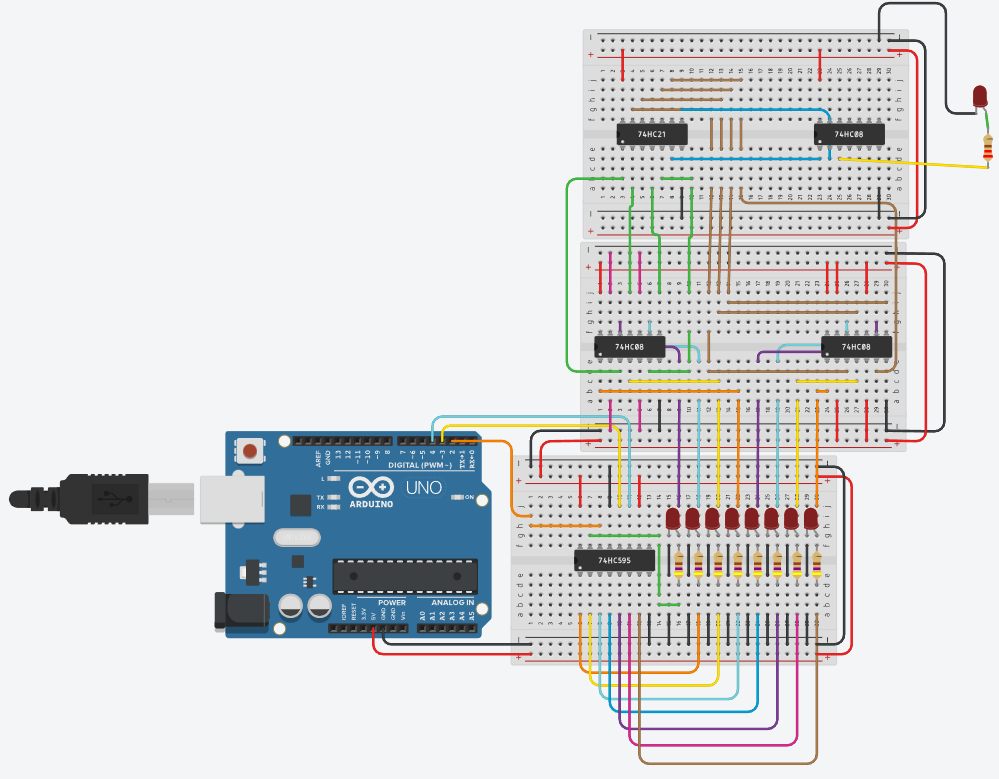
\includegraphics[scale=0.6]{74HC08.png}
\centering
\caption{Bloque de desencriptación hecho con compuertas AND.}
\label{fig:74HC08}
\end{figure}

Para comprobar el funcionamiento del sistema de desencriptación se tomó la clave asignada al grupo y se ingresó en el arreglo de tipo byte anteriormente mostrado en los códigos de conexión entre arduino. 
Se llegó a la conclusión, gracias a la tabla de verdad de la compuerta AND, que esta no era la indicada para la comparación de números que se requiere para que el sistema de desencriptación realice un trabajo exitoso.

Es necesario el uso de compuertas lógicas XOR que estén conectadas con compuertas lógicas NOT, las cuales nos dirán si el número binario que sale por el integrado 74HC595 de forma paralela es nuestra clave de desencriptación.

\newpage
\subsection{Prueba 2: Integrado 74HC86(XOR), 74HC04(NOT) 74HC21(AND4INPUTS), 74HC08(AND)}
Tras descubrir que la implementación de solo compuertas AND no era adecuada, se dibujó el circuito de compuertas lógicas para así saber claramente qué compuertas eran necesarias. El dibujo se presenta a continuación:

\begin{figure}[h]
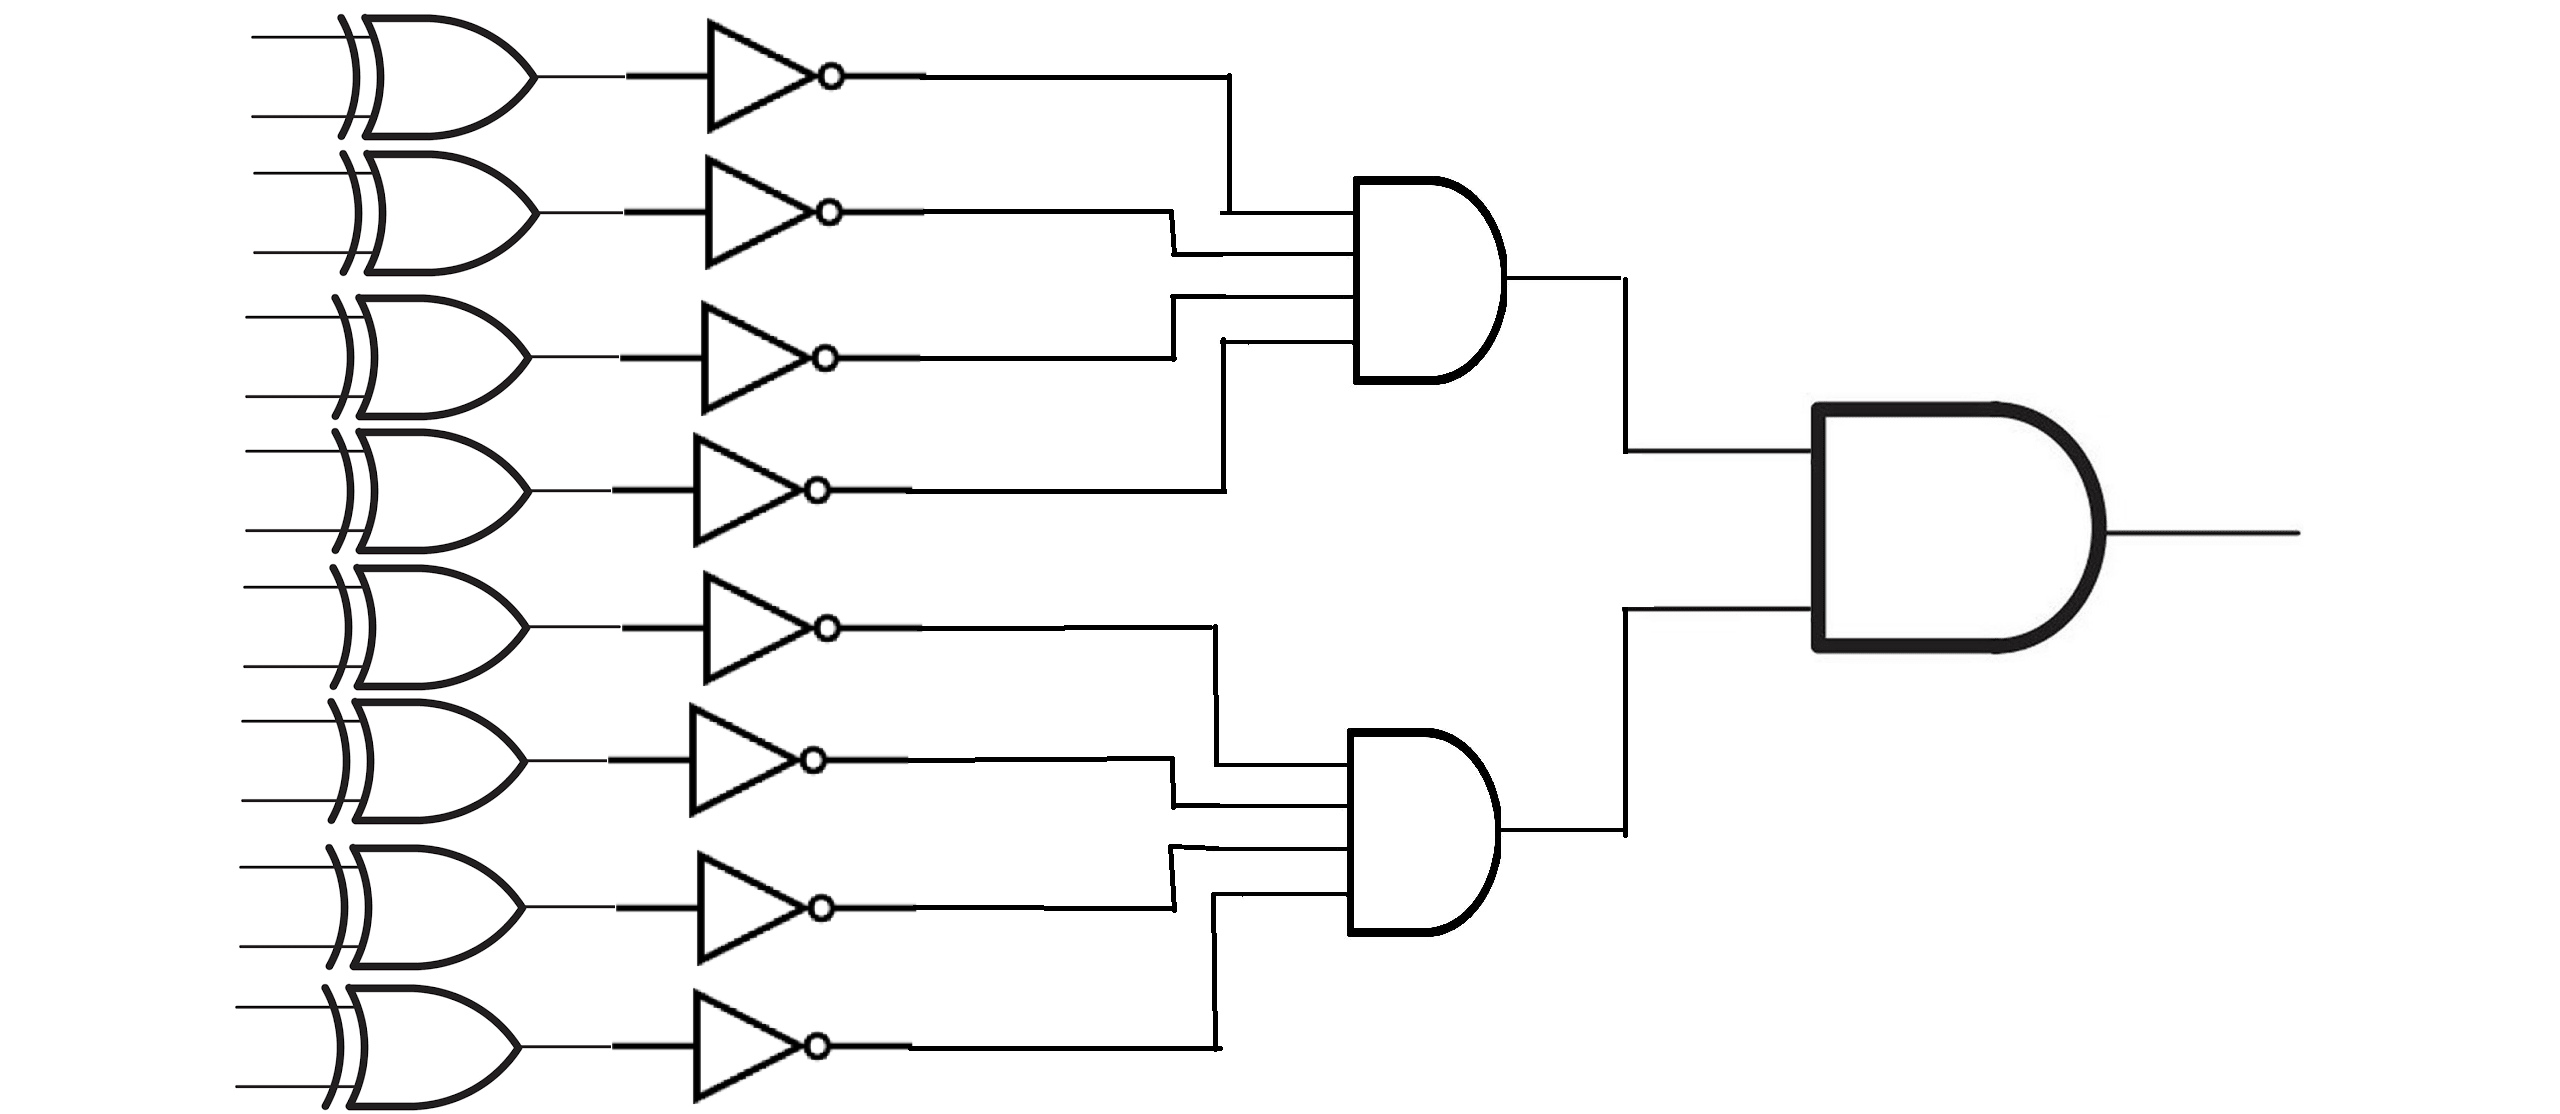
\includegraphics[scale=0.2]{compuertas.png}
\centering
\caption{Conexión de las compuertas necesarias para la comparación de números.}
\label{fig:compuertas}
\end{figure}

\begin{figure}[h]
\includegraphics[scale=0.8]{tablaVerdad.png}
\centering
\caption{Tablas de verdad de las compuertas XOR, AND y NOT.}
\label{fig:TablaVerdad}
\end{figure}

Las compuertas que recibirán la información bit a bit desde el circuito integrado 74HC6595 son las XOR, las cuales teniendo en cuenta su tabla de verdad Figura \ref{fig:TablaVerdad} nos arrojarán 1 cuando los datos sean diferentes y 0 cuando sean iguales, es por esto que a la salida de estas compuertas se hará necesario el uso de compuertas negadoras, para que cuando nuestros datos sean iguales obtengamos un uno y cuando sean diferentes obtengamos un cero. Estas salidas que obtenemos de las compuertas negadoras pasarán a las compuertas AND de cuatro entradas, esto porque necesitaremos saber si todas las salidas de las compuertas son uno, lo que confirmaría que el número ingresado a las compuertas XOR (integrado 74HC86) es la clave que estamos buscando. Por último, obtendremos dos salidas de las compuertas descritas anteriormente, estas dos salidas deberán entrar en otra AND de dos entradas la que nos mostrará uno (true) cuando sus dos datos de entrada sean 1, y cero (false) en cualquier otro caso. 


Después del análisis anterior se procedió al montaje con las compuertas en Tinkercad. Como podemos ver, se tomaron las salidas del integrado 74HC595 para ser comparadas en las compuertas XOR con la clave que necesitamos encontrar. La clave se ingresa en forma de binario con ayuda de GND (0) y Vcc (1), y se compara con las salidas del integrado 74HC595. Figura \ref{fig:desencriptación1}


\begin{figure}[h]
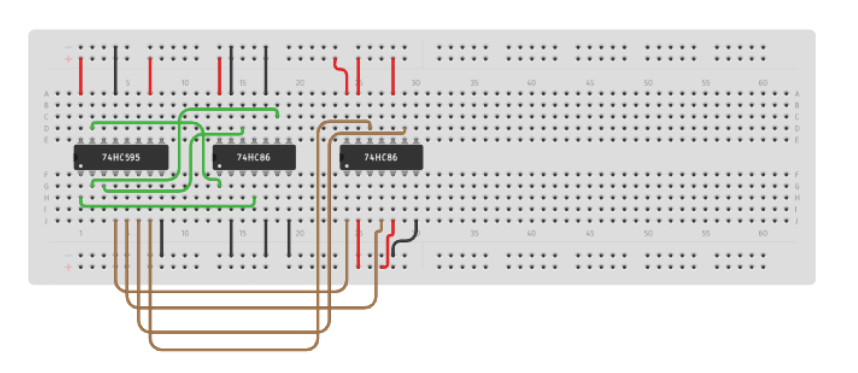
\includegraphics[scale=0.7]{desencriptacion1.png}
\centering
\caption{Inicio del montaje de desencriptación.}
\label{fig:desencriptación1}
\end{figure}

\newpage
Las salidas de las compuertas XOR pasan a los integrados 74HC04 para ser negadas, esto por la explicación que se dio anteriormente, y luego entran a las compuertas AND de cuatro entradas (74HC21) para comprobar que todas la comparaciones hayan sido verdaderas (entradas igual uno). Por último, se comprobará que las salidas del integrado 74HC21 sean verdaderas (uno), y de esta forma sabremos si el número ingresado a los integrados es la clave que estamos buscando.


\begin{figure}[h]
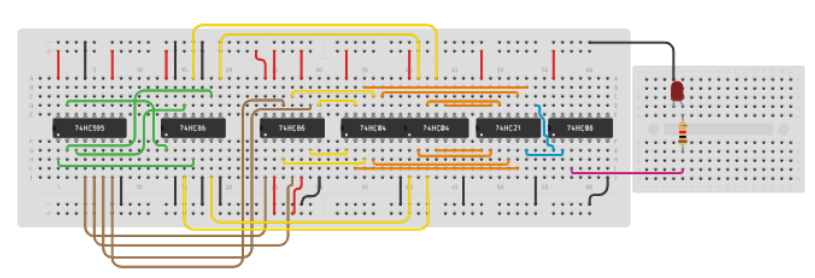
\includegraphics[scale=0.7]{desencriptacion2.png}
\centering
\caption{Montaje de desencriptación finalizado.}
\label{fig:desencriptación2}
\end{figure}

La verificación del funcionamiento de este sistema de comparación construido a partir de compuertas lógicas se realizó con dos pulsadores, un switch y una fuente de voltaje de 5v:

\newpage
\begin{figure}[h]
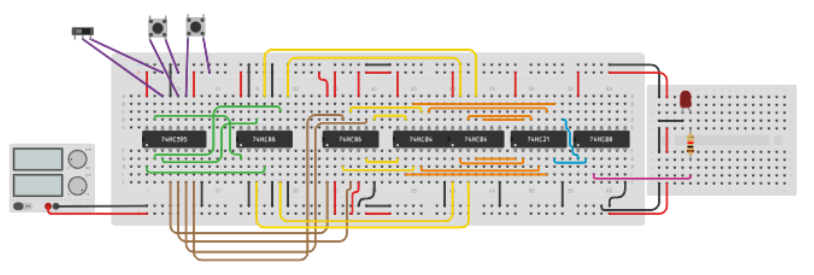
\includegraphics[scale=0.7]{desencriptacion pulsadores.png}
\centering
\caption{Montaje de desencriptación finalizado con pulsadores y fuente.}
\label{fig:desencriptación3}
\end{figure}

Afortunadamente, el circuito respondió tal como se esperaba, dando por finalizada la tarea de construir, en este caso, un desencriptador exitoso.


\section{Implementación sistema completo.} \label{sistema completo}

Se define el uso de dos arduinos, montados con sus respectivas placa base, arduino emisor el cual será el encargado de transmitir la información y arduino receptor quien nos indicará al momento de recibir la información desencriptada. El uso de la función "bintodec" la cual esta incluida en el codigo, fue clave, ya que nos permite convertir un binario a un decimal y de esta forma será la manera en la que transmitiremos los datos entre los arduinos.\newline
En el integrado se tiene un registro de 8 bits de dezplazamiento por cada salida, toma una entrada en serie a través de un solo pin y lo convierte en salida paralela de 8 bits reduciendo así eficazmente el número de pines de interfaz entre un Microcontrolador y sus dispositivosde salida
En el registro de desplazamiento tenemos una entrada en serie y datos en paralelos (salida), con cada pulso se comienza el progreso o 
ingreso de los datos en serie SER, reloj (SRCLK).\newline
Los tres pines del registro de turnos que se necesitan para conectarse a Arduino son los pines 11 (la entrada del reloj), 12 (la entrada del reloj del registro de almacenamiento o simplemente la entrada del pestillo) y 14 (laentradade datos).
A continuación se presenta la integración del bloque de desencriptación y la comunicación entre arduinos:

\newpage
\subsection{Implementación sistema completo con salida en monitor serial}\label{intento1}
Inicialmente se optó por implementarlo mostrando la salida por medio del monitor serial, para así poder confirmar su funcionamiento sin el riesgo que el error se encuentre en la conexión de los cables al lcd.


montaje:
\begin{figure}[h]
\includegraphics[scale=0.5]{integracion arduinos serial.png}
\centering
\caption{Integración del bloque de desencriptación, mostrando la información mediante el monitor serial}
\label{fig:serial}
\end{figure}

Código emisor:
\begin{lstlisting}[style=myArduino]
//directivas de preprocesamiento
#define TIEMPO 1000
#define SER 2
#define RCLK 3
#define SRCLK 4


byte codigo[30];
//A byte stores an 8-bit unsigned number, from 0 to 255.
int tamanoArray=sizeof(codigo)/sizeof(byte);
//----------------------------------------------------------------
//prototipo de las funciones

//----------------------------------------------------------------
//setup
void setup()
{
  for(int i=2;i<5;i++)
  {
    pinMode(i, OUTPUT);
    digitalWrite(i, LOW);
  }
  
  //ensayo
  for(int i=0;i<30;i++)
  {
    codigo[i]=i+14;
  }
}
//----------------------------------------------------------------
//loop
void loop()
{
  for(int i=0;i<tamanoArray;i++)
  {
    for(int j=0;j<8;j++)
    {
      digitalWrite(SER, bitRead(codigo[i], j));
      digitalWrite(SRCLK, HIGH);
      delay(100);
      digitalWrite(SRCLK, LOW);

    }
    delay(TIEMPO);
    digitalWrite(RCLK, HIGH);
    digitalWrite(RCLK, LOW);
    
  }
  
  
  
}
//----------------------------------------------------------------
//cuerpo de las funciones
\end{lstlisting}

Código receptor:
\begin{lstlisting}[style=myArduino]
#define SER 2
#define RCLK 3
#define SRCLK 4
#define TIEMPO 1000
#define CLAVE 5

//byte codigo[]={1,2,255,0,15,6,7,8};
//byte codigo[]={15,15,255,0,15,15,7,8};
byte binario[8];

byte bintodec(byte* bin);
byte dos_exp (int exp);

bool contar=false;
int posicion=-1;

void setup()
{
  Serial.begin(9600);
  for(int i=2;i<6;i++)
  {
    pinMode(i, INPUT);
  }
}

void loop()
{
  
  if(digitalRead(SRCLK))
  {
    for(int i=0;i<8;i++)
    {
      while(!digitalRead(SRCLK))
      {
        
      }
      binario[i]=digitalRead(SER);
      while(digitalRead(SRCLK))
      {
        
      }
    }
    
    delay(TIEMPO);
    for(int i=7;i>=0;i--)
    {
      Serial.print(binario[i]);
    }
    Serial.println();
    Serial.println(bintodec(binario));
    
    if(digitalRead(CLAVE))
    {
      contar=true;
      Serial.println("se leyo la clave");
    }
    
   	if(contar)
    {
      posicion++;
      Serial.print("posicion= ");
      Serial.println(posicion);
    }
    if(posicion==3)
    {
      Serial.println("hola");
      contar=false;
      posicion=-1;
    }
  }
}
//--------------------------------------------------------------
//funciones
byte bintodec(byte * bin){ // recibe un binario y retorna un decimal en tipo entero
    byte dec = 0;
    for(int i=7; i>=0 ; i--){
        if (bin[i]>=1){
                dec = dec + (dos_exp(i));
        }
    }
    return dec;
}

byte dos_exp (int exp){
    int acu = 1;
    for (int i=0 ; i<exp ; i++){
        acu = acu*2;
    }
    return acu;
}
\end{lstlisting}

\subsection{Implementación sistema completo con salida en monitor serial y LCD}\label{intento1}
Una vez se confirmó que no había ningún error, se procedió a implementarlo tanto en monitor serial como en el display lcd, para así poder verificar que la salida del serial coincida con la mostrada en el lcd.

montaje:
\begin{figure}[h]
\includegraphics[scale=0.5]{integracion arduinos serial y lcd.png}
\centering
\caption{Integración del bloque de desencriptación, mostrando la información mediante el monitor serial y el lcd}
\label{fig:serialLcd}
\end{figure}

Código emisor:
\begin{lstlisting}[style=myArduino]
//directivas de preprocesamiento
#define TIEMPO 1000
#define SER 2
#define RCLK 3
#define SRCLK 4


byte codigo[30];
//A byte stores an 8-bit unsigned number, from 0 to 255.
int tamanoArray=sizeof(codigo)/sizeof(byte);
//----------------------------------------------------------------
//prototipo de las funciones

//----------------------------------------------------------------
//setup
void setup()
{
  for(int i=2;i<5;i++)
  {
    pinMode(i, OUTPUT);
    digitalWrite(i, LOW);
  }
  
  //ensayo
  for(int i=0;i<30;i++)
  {
    codigo[i]=i+14;
  }
}
//----------------------------------------------------------------
//loop
void loop()
{
  for(int i=0;i<tamanoArray;i++)
  {
    for(int j=0;j<8;j++)
    {
      digitalWrite(SER, bitRead(codigo[i], j));
      digitalWrite(SRCLK, HIGH);
      delay(100);
      digitalWrite(SRCLK, LOW);

    }
    delay(TIEMPO);
    digitalWrite(RCLK, HIGH);
    digitalWrite(RCLK, LOW);
    
  }
  
  
  
}
//----------------------------------------------------------------
//cuerpo de las funciones
\end{lstlisting}

Código receptor serial:
\begin{lstlisting}[style=myArduino]
#define SER 2
#define RCLK 3
#define SRCLK 4
#define TIEMPO 1000
#define CLAVE 5

//byte codigo[]={1,2,255,0,15,6,7,8};
//byte codigo[]={15,15,255,0,15,15,7,8};
byte binario[8];

byte bintodec(byte* bin);
byte dos_exp (int exp);

bool contar=false;
int posicion=-1;

void setup()
{
  Serial.begin(9600);
  for(int i=2;i<6;i++)
  {
    pinMode(i, INPUT);
  }
}

void loop()
{
  
  if(digitalRead(SRCLK))
  {
    for(int i=0;i<8;i++)
    {
      while(!digitalRead(SRCLK))
      {
        
      }
      binario[i]=digitalRead(SER);
      while(digitalRead(SRCLK))
      {
        
      }
    }
    
    delay(TIEMPO);
    for(int i=7;i>=0;i--)
    {
      Serial.print(binario[i]);
    }
    Serial.println();
    Serial.println(bintodec(binario));
    
    if(digitalRead(CLAVE))
    {
      contar=true;
      Serial.println("se leyo la clave");
    }
    
   	if(contar)
    {
      posicion++;
      Serial.print("posicion= ");
      Serial.println(posicion);
    }
    if(posicion==3)
    {
      Serial.println("hola");
      contar=false;
      posicion=-1;
    }
  }
}
//--------------------------------------------------------------
//funciones
byte bintodec(byte * bin){ // recibe un binario y retorna un decimal en tipo entero
    byte dec = 0;
    for(int i=7; i>=0 ; i--){
        if (bin[i]>=1){
                dec = dec + (dos_exp(i));
        }
    }
    return dec;
}

byte dos_exp (int exp){
    int acu = 1;
    for (int i=0 ; i<exp ; i++){
        acu = acu*2;
    }
    return acu;
}
\end{lstlisting}

Código receptor lcd:
\begin{lstlisting}[style=myArduino]
// include the library code:
#include <LiquidCrystal.h>

// initialize the library with the numbers of the interface pins
LiquidCrystal lcd(12, 11, 5, 4, 3, 2);

#define SER 7
#define RCLK 8
#define SRCLK 9
#define CLAVE 10
#define TIEMPO 1000

byte bintodec(byte * bin);
byte binario[8];

byte dos_exp (int exp);

bool contar=false;
int posicion=-1;

void setup() {
  // set up the LCD's number of columns and rows:
  lcd.begin(16, 2);
  
  for(int i=7;i<11;i++)
  {
    pinMode(i, INPUT);
  }
}

void loop() {
  
  if(digitalRead(SRCLK))
  {
    for(int i=0;i<8;i++)
    {
      while(!digitalRead(SRCLK))
      {
        
      }
      //Serial.print(digitalRead(2));
      binario[i]=digitalRead(SER);
      while(digitalRead(SRCLK))
      {
        
      }
    }
    delay(TIEMPO);
    lcd.clear();
    for(int i=7;i>=0;i--)
    {
      lcd.print(binario[i]);
    }
    lcd.setCursor(0, 1);
    lcd.print(bintodec(binario));
    
	if(digitalRead(CLAVE))
    {
      contar=true;
      lcd.print("se leyo la clave");
    }
    
   	if(contar)
    {
      posicion++;
      lcd.print("posicion= ");
      lcd.print(posicion);
    }
    if(posicion==3)
    {
      lcd.print("hola");
      contar=false;
      posicion=-1;
    }

  }
  
}


//funciones
byte bintodec(byte * bin){ // recibe un binario y retorna un decimal en tipo entero
    byte dec = 0;
    for(int i=7; i>=0 ; i--){
        if (bin[i]>=1){
                dec = dec + (dos_exp(i));
        }
    }
    return dec;
}

byte dos_exp (int exp){
    int acu = 1;
    for (int i=0 ; i<exp ; i++){
        acu = acu*2;
    }
    return acu;
} 
\end{lstlisting}

El sistema se comportó tal como se esperaba tanto en el monitor serial como en el display LCD.

\newpage
\subsection{Implementación sistema completo con salida en display LCD (SISTEMA FINALIZADO)}\label{intento1}
Ya que el montaje del display funcionó correctamente, se procedió a eliminar el arduino encargado del monitor serial. Y para que el proyecto tenga un mejor acabado, se procedió a segmentar el código, y comentarlo de una forma más estructurada, a su vez, eliminando todo lo no necesario para el funcionamiento correcto del sistema:

montaje:
\begin{figure}[h]
\includegraphics[scale=0.5]{integracion arduinos lcd.png}
\centering
\caption{Integración del bloque de desencriptación, mostrando la información mediante el display lcd.}
\label{fig:lcd}
\end{figure}

Código emisor:
\begin{lstlisting}[style=myArduino]
//DIRECTIVAS DE PREPROCESAMIENTO

#define TIEMPO 500
#define SER 2
#define RCLK 3
#define SRCLK 4
#define TAMANO 60

//--------------------------------------------------------------
//--------------------------------------------------------------
//ARREGLOS DE PRUEBA (descomente uno solo a la vez):

byte codigo[]={15,15,255,0,15,15,7,8,15,9,2,15};
//byte codigo[]={1,2,255,0,15,6,7,8};

//En caso de querer crear un arreglo mediante un ciclo for:
//byte codigo[TAMANO];
//1.Cambie el tamano del arreglo en la directiva de
//preprocesamiento llamada TAMANO en la linea: 7.
//2.Quite los comentarios del for ubicado en la linea: 45
//y modifique como funcionará este para llenar el arreglo.

//¿Por qué el tipo byte?
//A byte stores an 8-bit unsigned number, from 0 to 255.

//--------------------------------------------------------------
//--------------------------------------------------------------
//VARIABLES:

int tamanoArray=sizeof(codigo)/sizeof(byte);

//--------------------------------------------------------------
//--------------------------------------------------------------
//setup

void setup()
{
  //configuramos los puertos de salida y los inicializamos en 0
  for(int i=2;i<5;i++)
  {
    pinMode(i, OUTPUT);
    digitalWrite(i, LOW);
  }
  
  //ARREGLO MODIFICABLE:
  /*for(int i=0;i<TAMANO;i++)
  {
    if(i<=30)
    {
      codigo[i]=i+14;
    }
    else if(i>32)
    {
      codigo[i]=i+100;
    }
    else
    {
      codigo[i]=15;
    }
  }*/
}

//--------------------------------------------------------------
//--------------------------------------------------------------
//loop

void loop()
{
  //recorremos cada elemento
  for(int i=0;i<tamanoArray;i++)
  {
    //obtenemos los 8 bits
    for(int j=0;j<8;j++)
    {
      digitalWrite(SER, bitRead(codigo[i], j));//j=0 menos signi
      digitalWrite(SRCLK, HIGH);
      delay(100);
      digitalWrite(SRCLK, LOW);
    }
    delay(TIEMPO);
    digitalWrite(RCLK, HIGH);
    digitalWrite(RCLK, LOW); 
  } 
}
\end{lstlisting}

Código receptor:
\begin{lstlisting}[style=myArduino]
//LIBRERIAS Y SU INICIALIZACION:

#include <LiquidCrystal.h>
// initialize the library with the numbers of the interface pins
LiquidCrystal lcd(12, 11, 5, 4, 3, 2);

//--------------------------------------------------------------
//--------------------------------------------------------------
//DIRECTIVAS DE PREPROCESAMIENTO:

#define SER 7
#define RCLK 8
#define SRCLK 9
#define CLAVE 10
#define TIEMPO 500

//--------------------------------------------------------------
//--------------------------------------------------------------
//PROTOTIPO DE LAS FUNCIONES:

byte bintodec(byte * bin);
byte dos_exp (int exp);

//--------------------------------------------------------------
//--------------------------------------------------------------
//VARIABLES Y ARREGLOS:

bool contar=false;
int posicion=0;
byte binario[8];

//--------------------------------------------------------------
//--------------------------------------------------------------
//setup

void setup() 
{
  // set up the LCD's number of columns and rows:
  lcd.begin(16, 2);
  //configuramos los puertos de entrada
  for(int i=7;i<11;i++)
  {
    pinMode(i, INPUT);
  }
}

//--------------------------------------------------------------
//--------------------------------------------------------------
//loop

void loop() 
{
  //si se envia un digito
  if(digitalRead(SRCLK))
  {
    //verifica si se recibe la clave
    if(digitalRead(CLAVE))
    {
      contar=true;
    }
    //guarda los 8 bits recibidos
    for(int i=0;i<8;i++)
    {
      while(!digitalRead(SRCLK))
      {
        
      }
      binario[i]=digitalRead(SER);
      while(digitalRead(SRCLK))
      {
        
      }
    }
    delay(TIEMPO);
 	//si recibio la clave, comienza a contar
   	if(contar)
    {
      posicion++;
    }
    //si van 15 posiciones luego de recibir la clave
    if(posicion==15)
    {
      lcd.clear();
      lcd.print(bintodec(binario));//muestra el numero secreto
      //lcd.print("-");
      contar=false;
      posicion=0;
    }
  }
}

//--------------------------------------------------------------
//--------------------------------------------------------------
//FUNCIONES:

// recibe un binario y retorna un decimal en tipo entero
byte bintodec(byte * bin){ 
    byte dec = 0;
    for(int i=7; i>=0 ; i--){
        if (bin[i]>=1){
                dec = dec + (dos_exp(i));
        }
    }
    return dec;
}

byte dos_exp (int exp){
    int acu = 1;
    for (int i=0 ; i<exp ; i++){
        acu = acu*2;
    }
    return acu;
} 
\end{lstlisting}

El sistema completo funciona correctamente y puede ser probado haciendo uso del siguiente link: 

\url{https://www.tinkercad.com/things/6DJhzwBksef}


\section{Conclusiones} \label{conclusiones}

\begin{itemize}
    \item El uso del integrado 74HC595 fue clave para la solución del problema, pues nos permitió paralelizar los datos que llegaban en serie, de esta forma se minimizó el uso de puertos digitales en el arduino receptor y se ingresó el número a desencriptar al bloque de desencriptación para ser comparado con la clave asignada.
    \item Para lograr una conexión entre arduinos exitosa se necesitó comprender el uso del circuito integrado 74HC595, ya que la sincronización entre el arduino emisor y receptor se logró gracias al SRLCK (Reloj de registro de desplazamiento), y al RCLK (Reloj de registro de salida).
    
    
    
\end{itemize}



\section{Cibergrafía} \label{ciber}

https://www.electrogeekshop.com/como-funciona-el-74hc595-shift-register-y-su-interfaz-con-arduino/
\newline
https://github.com/trihedral/ArduinoLatexListing
\newline
https://www.youtube.com/watch?v=9gfZnNPBlVg

\end{document}
